\section{Experiments and Results}
\label{sec:results}

\subsection{Baseline and Full-Measurement Benchmark}
Table~\ref{tab:main} reports the three models under full measurement availability. The
median baseline attains $R^2 = -0.092$, confirming that a constant predictor is worse
than useless on this target. Both ensembles exceed it by a wide margin, with XGBoost
reaching $R^2 = 0.9997$ and a mean absolute error of 0.100 index points. Throughout, the
two ensembles are trained on unequal budgets -- Random Forest on a 100{,}000-record
subsample, XGBoost on the full 1{,}986{,}397-record partition
(Section~\ref{sec:models}) -- so the margin between them is not a clean algorithmic
comparison and should be read with that in mind.

This near-perfect score should be read as what it is. By Equation~\eqref{eq:ccme} the
target is determined by the inputs, so the result measures how well a tree ensemble
approximates a known piecewise function. We report it as a benchmark and as a check on
the pipeline: a materially lower score here would indicate a defect upstream.

\begin{table}[!t]
    \centering
    \caption{Phase 1 model comparison on the held-out test set, all-measurements regime; all figures are test-set. The baseline predicts the training median; Random Forest is fitted on a 100k subsample and XGBoost on the full training partition, both with engineered features.}
    \label{tab:main}
    \small
    \setlength{\tabcolsep}{4pt}
    \begin{tabular}{lrrrr}
        \toprule
        Model & MAE & RMSE & $R^2$ & Train (s) \\
        \midrule
        Naive baseline & 13.605 & 19.492 & -0.0923 & 0.0 \\
        Random Forest & 0.408 & 0.920 & 0.9976 & 1.7 \\
        XGBoost & 0.100 & 0.328 & 0.9997 & 49.3 \\
        \bottomrule
    \end{tabular}
\end{table}


\subsection{Partial Measurement Availability}
Table~\ref{tab:partial} and Fig.~\ref{fig:degradation} give the central result.
Withholding a single measurement moves XGBoost from $R^2 = 0.9997$ to $0.834$, and mean
absolute error from 0.100 to 4.776 -- a factor of 48. Withholding four leaves
$R^2 = 0.573$ and an error of 8.596 index points, which spans roughly one CCME quality
class. XGBoost leads Random Forest at every level, and the margin is stable at
2--4\% of $R^2$ despite the twentyfold difference in training-set size, which suggests
the ordering is not purely a budget effect even though its magnitude is not separable
from one.

The gap between the 8/8 and 7/8 rows is the quantitative statement of the leakage
problem. Almost all of the apparent accuracy in the full-measurement setting comes from
the formula being reconstructible, not from any learned relationship that survives when
an input is withdrawn.

\begin{table*}[!t]
    \centering
    \caption{Degradation under partial measurement availability. The 8/8 row is a formula-emulation benchmark, not independent prediction; genuine estimation begins at 7/8. $p$ is the feature count after masking; all figures are test-set.}
    \label{tab:partial}
    \small
    \setlength{\tabcolsep}{4pt}
    \begin{tabular}{llrrrr}
        \toprule
        Avail. & Model & $p$ & MAE & RMSE & $R^2$ \\
        \midrule
        8/8 & Random Forest & 38 & 0.408 & 0.920 & 0.9976 \\
        8/8 & XGBoost & 23 & 0.100 & 0.328 & 0.9997 \\
        7/8 & Random Forest & 35 & 5.328 & 8.145 & 0.8093 \\
        7/8 & XGBoost & 20 & 4.776 & 7.597 & 0.8341 \\
        6/8 & Random Forest & 32 & 5.675 & 8.544 & 0.7901 \\
        6/8 & XGBoost & 17 & 5.209 & 8.045 & 0.8139 \\
        4/8 & Random Forest & 25 & 9.305 & 12.781 & 0.5304 \\
        4/8 & XGBoost & 10 & 8.596 & 12.190 & 0.5728 \\
        \bottomrule
    \end{tabular}
\end{table*}


\begin{figure}[!t]
    \centering
    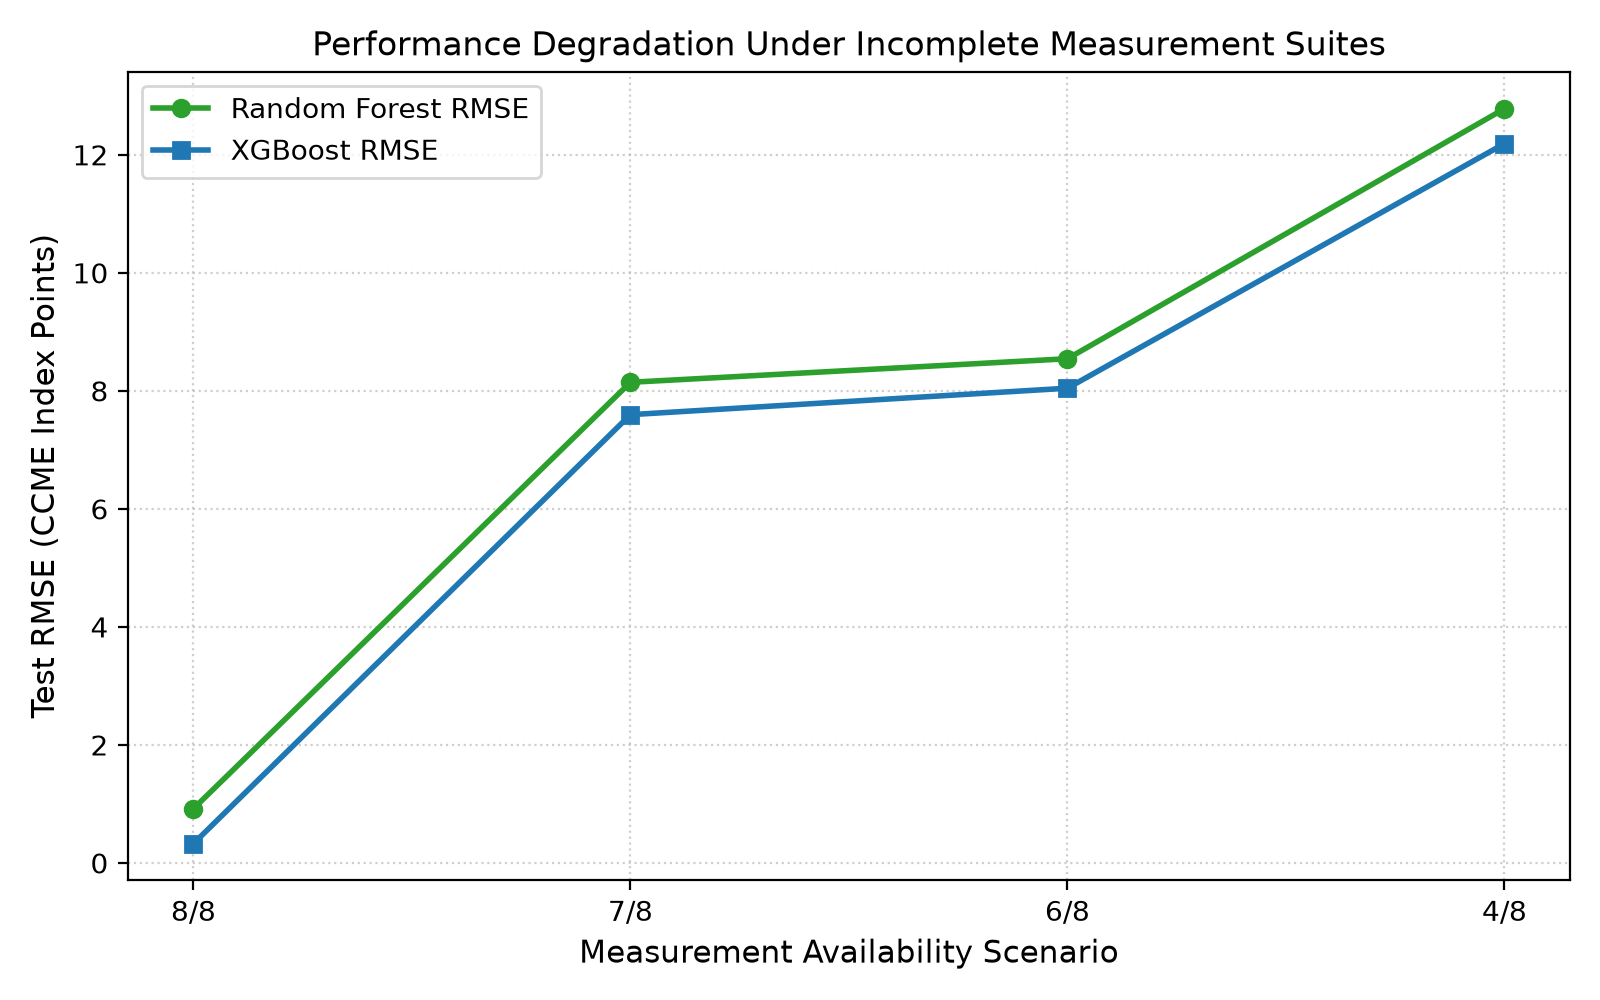
\includegraphics[width=\linewidth]{06_partial_measurement_degradation.png}
    \caption{Test performance against measurement availability. The step between 8/8 and
    7/8 isolates the contribution of formula reconstruction.}
    \label{fig:degradation}
\end{figure}

\subsection{Ablations}
Table~\ref{tab:ablation} isolates two design choices. Engineered features reduce XGBoost
test MAE from 0.1517 to 0.1000, a 34\% relative improvement, confirming that the
logarithmic transforms and chemical ratios carry information beyond the raw columns.
Adding the upstream-imputation flags changes test MAE only from 0.1517 to 0.1474. Given
their confounding with country (Section~\ref{sec:imputation}), this small gain does not
justify their inclusion, and we exclude them from the primary configuration.

\begin{table*}[!t]
    \centering
    \caption{Ablation studies on XGBoost, all-measurements regime. $p$ is the feature count; all figures are test-set.}
    \label{tab:ablation}
    \small
    \setlength{\tabcolsep}{4pt}
    \begin{tabular}{lllrrr}
        \toprule
        Ablation & Config. & $p$ & MAE & RMSE & $R^2$ \\
        \midrule
        Imputation flags & Excluded (primary) & 10 & 0.1517 & 0.4005 & 0.99954 \\
        Imputation flags & Included & 20 & 0.1474 & 0.3979 & 0.99954 \\
        Features & Raw & 10 & 0.1517 & 0.4005 & 0.99954 \\
        Features & Raw + engineered & 23 & 0.1000 & 0.3282 & 0.99969 \\
        \bottomrule
    \end{tabular}
\end{table*}


\subsection{Uncertainty and Error Decomposition}
Table~\ref{tab:bootstrap} gives bootstrap confidence intervals. The intervals for Random
Forest and XGBoost do not overlap on any metric, so the ordering between them is not an
artefact of sampling.

Table~\ref{tab:country} decomposes test error by country over all 415{,}804 test
records. Performance is uniformly high in the full-measurement regime, but the sample
sizes are extremely unequal: England supplies 76.8\% of test records and Canada 0.14\%,
so the Canadian figures rest on 584 records and should not be read as a country-level
comparison. England's share of the test set (76.8\%) differs slightly from its share of
the corpus (75.3\%) because whole sites are allocated to partitions, so the split
matches the target proportions only as closely as integer site sizes permit. China is
absent: its single site is allocated wholly to training (Section~\ref{sec:split}), so it
contributes no test records and cannot be evaluated out-of-sample.

\begin{table*}[!t]
    \centering
    \caption{Bootstrap point estimates with 95\% confidence intervals on the test set.}
    \label{tab:bootstrap}
    \small
    \setlength{\tabcolsep}{4pt}
    \begin{tabular}{lllp{0.28\linewidth}}
        \toprule
        Model & MAE (Point [95\% CI]) & RMSE (Point [95\% CI]) & R2 (Point [95\% CI]) \\
        \midrule
        Naive Baseline & 13.6047 [13.5631, 13.6457] & 19.4916 [19.4378, 19.5410] & -0.0923 [-0.0936, -0.0907] \\
        Random Forest & 0.4078 [0.4053, 0.4103] & 0.9197 [0.9102, 0.9297] & 0.9976 [0.9975, 0.9976] \\
        XGBoost & 0.1000 [0.0991, 0.1009] & 0.3282 [0.3228, 0.3337] & 0.9997 [0.9997, 0.9997] \\
        \bottomrule
    \end{tabular}
\end{table*}

\begin{table}[!t]
    \centering
    \caption{Test error decomposed by country, over all 415{,}804 test records. China is absent by construction: its single site (Hou Bay) is allocated wholly to training, so it contributes no test records and cannot be evaluated out-of-sample.}
    \label{tab:country}
    \small
    \setlength{\tabcolsep}{4pt}
    \begin{tabular}{lrrrrr}
        \toprule
        Country & $n$ & \% of test & MAE & RMSE & $R^2$ \\
        \midrule
        England & 319184 & 76.76 & 0.116 & 0.329 & 0.9997 \\
        USA & 60787 & 14.62 & 0.062 & 0.394 & 0.9937 \\
        Ireland & 35249 & 8.48 & 0.019 & 0.123 & 0.9996 \\
        Canada & 584 & 0.14 & 0.176 & 0.561 & 0.9982 \\
        \bottomrule
    \end{tabular}
\end{table}


\subsection{Feature Attribution}
Table~\ref{tab:shap} ranks features by mean absolute SHAP value. Orthophosphate dominates
at 8.813, nearly three times the next contributor, which matches both its Spearman
correlation of $-0.917$ and its position in Equation~\eqref{eq:ccme}: it carries the
tightest guideline threshold and therefore the largest excursion term. The appearance of
the engineered logarithmic transforms in the top five corroborates the ablation.

\begin{table}[!t]
    \centering
    \caption{Ten most influential features by mean absolute SHAP value (XGBoost, 8/8 regime).}
    \label{tab:shap}
    \small
    \setlength{\tabcolsep}{4pt}
    \begin{tabular}{lr}
        \toprule
        Feature & Mean $|$SHAP$|$ \\
        \midrule
        Orthophosphate (mg/l) & 8.813 \\
        log\_Orthophosphate & 3.062 \\
        Ammonia (mg/l) & 2.455 \\
        Biochemical Oxygen Demand (mg/l) & 1.061 \\
        log\_Ammonia & 0.691 \\
        Nitrogen (mg/l) & 0.267 \\
        pH (ph units) & 0.229 \\
        log\_BOD & 0.178 \\
        Temperature (cel) & 0.160 \\
        N\_P\_ratio & 0.110 \\
        \bottomrule
    \end{tabular}
\end{table}


\begin{figure}[!t]
    \centering
    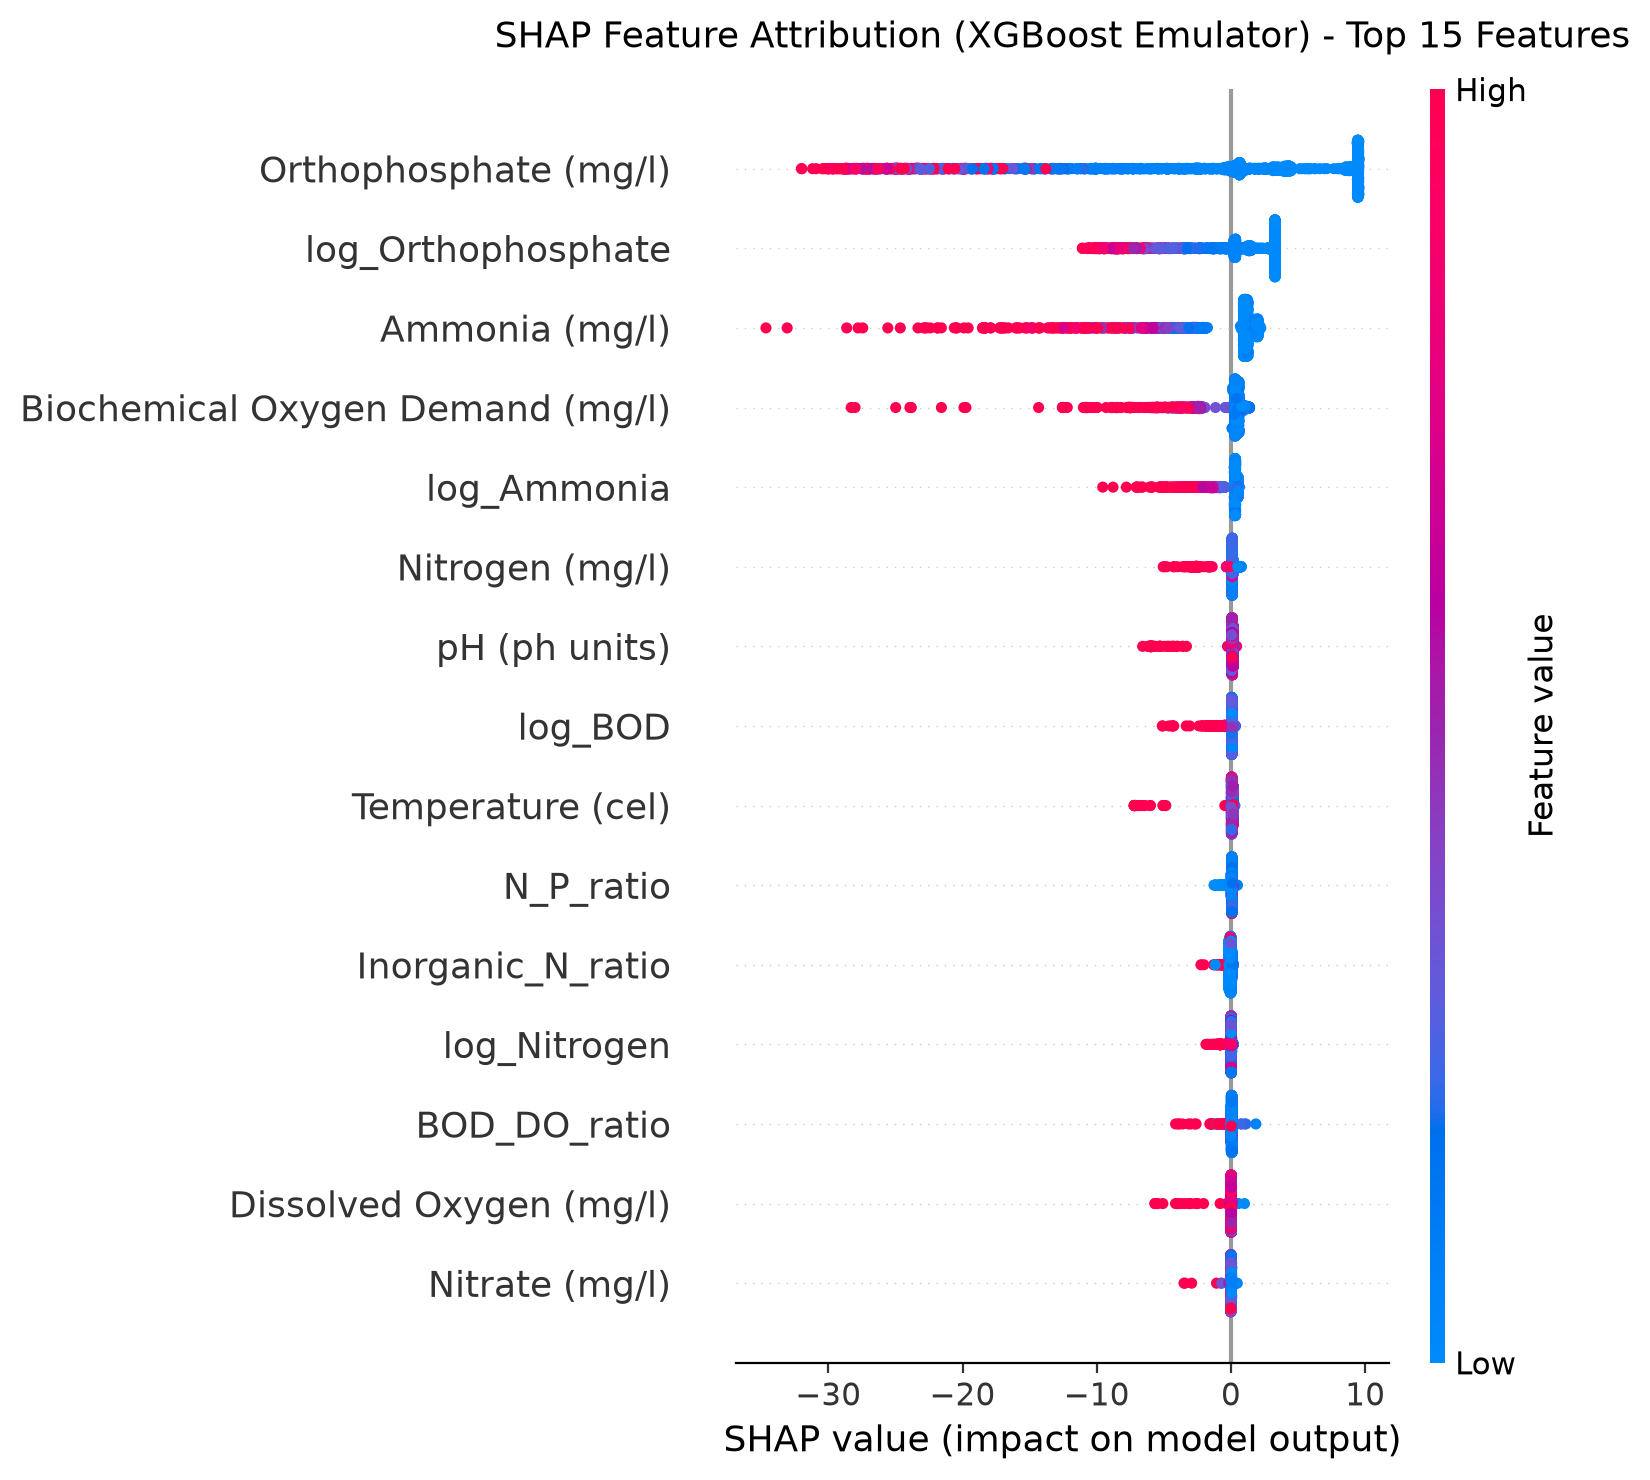
\includegraphics[width=\linewidth]{06_shap_summary.png}
    \caption{SHAP summary for the full-measurement XGBoost model.}
    \label{fig:shap}
\end{figure}
